\documentclass{article}
\usepackage{polski}
\usepackage{listings}
\usepackage{pgfplots}
\usepackage{hyperref}
\usepackage{graphicx}
\usepackage{subfigure}
\usepackage[margin=4cm]{geometry}

\graphicspath{ {./images/} }

\pgfplotsset{compat=1.18}
\usepgfplotslibrary{statistics}

\lstset{
	tabsize=2,
	basicstyle=\ttfamily,
  columns=fullflexible,
  keepspaces=true,
	frame=tb,
	%numbers=left
}

\newcommand{\includeplots}[1]{
\begin{figure*}[htp]
\centering
	\subfigure[Histogram błędu pomiędzy zbiorem testowym, a odpowiadającymi mu predykcjami]{
		\includegraphics[scale=0.45]{#1.hist.png}
	}
	\subfigure[Porównanie predykcji wartości ocen z wartościami testowymi]{
		\includegraphics[scale=0.45]{#1.scatter.png}
	}
\end{figure*}
}

\newcommand{\sql}[2]{
\lstinputlisting[language=SQL,caption=#1]{#2}
}

\title{Predykcja ocen filmów oraz seriali\\ \large Projekt w ramach laboratoriów Przetwarzania Języka Naturalnego}
\author{Robert Bendun}
\date{2022-01-10}

\begin{document}

\maketitle

\tableofcontents

\pagebreak

\section{Informacje ogólne}

\subsection{Metodyka pracy} \label{metodyka}

Oparta jest o zbiór programów stworzonych na rzecz tego projektu oraz narzędzi \href{https://www.gnu.org/software/coreutils/}{GNU Coreutils}. Konstrukcja programów, skryptów itp. ma na celu stworzenie środowiska pozwalającego na pracę w duchu \href{https://en.wikipedia.org/wiki/Unix_philosophy}{filozofii Unixa}.

Równie ważnym celem poza reakcją samego projektu było (zainspirowane interfejsem terminalowym Vowpala Wabbita) stworzenie fremeworku do prostego tworzenia, operowania oraz łączenia zbiorów danych o podobnej tematyce.

\subsubsection{Programy}

\begin{itemize}
\item \textbf{bin/db-tool} Narzędzie umożliwiające interakcję ze zbiorem danych przechowywanym w bazie SQL.
	\begin{itemize}
		\item \textbf{bin/db-tool import} Importuje dane TSV do tabeli wewnątrz bazy danych SQL
		\item \textbf{bin/db-tool vw} Generuje plik Vovpal Wabbit wg kwerendy używającej rozszerzonego SQL
	\end{itemize}
\item \textbf{bin/metrics} - Generuje wyniki ewaluacji modelu na podstawie zbioru predykcji oraz testowego
\item \textbf{bin/psplit} - Dzieli proporcjonalnie i losowo wg wag zbiór danych
\item \textbf{progs/error-hist.py} - Generuje histogram błędu pomiędzy zbiorem testowym a predykcjami
\end{itemize}

\subsubsection{Rozszerzenie języka SQL}

Pozwala opisywać zbiory danych przy pomocy pojedyńczych kwerend SQL. Rozszerza przy pomocy \href{https://pkg.go.dev/go}{parsera języka Go}, poprzez mechanizm nazw kolumn. Lista dostępnych komend zdefiniowana jest w progs/db-tool/action/action.go. Jest używana do precyzyjniejszego opisu zbiorów używanych w danych predykcjach.

\subsection{Zbiór danych}

\subsubsection{Dane z serwisu IMDB}

IMDB udostępnia gotowe zbiory danych (będące podzbiorem ogólnych informacji w serwisie), dostępne do pobrania w formie skompresowanych plików TSV. Wykorzystuję je bezpośrednio jako źródła tabel, na których operuję poniżej.

\begin{center}
\begin{tabular}{ |c|c| p{0.6\linewidth} | }
	\hline
	\textbf{Nazwa tabeli} & \textbf{Plik źródłowy} & \textbf{Opis zawartości} \\ \hline
	Basics & title.basics.tsv.gz & Podstawowe informacje na temat pozycji w katalogu IMDB, takie jak nazwa filmu, rok produkcji, długość czy gatunek \\ \hline
	Episodes & title.episode.tsv.gz & Wiąże seriale wraz z ich epizodami \\ \hline
	Names & name.basics.tsv.gz & Imię, nazwisko, data urodzenia (opcjonalnie róœnież śmierci) osoby występującej w tabeli Principals \\ \hline
	Principals & title.principals.tsv.gz & Główna obsada oraz osoby zaangażowane w produkcję danego dzieła \\ \hline
	Ratings & title.ratings.tsv.gz & Ocena filmu oraz liczba kont głosujących \\ \hline
\end{tabular}
\end{center}

\section{Predykcje oparte o proste podzbiory wartości}

Działania w tej sekcji miały na celu wyznaczyć minimalny poziom akceptowalnych predykcji. Jakiekolwiek bardziej złożone konstrukcje nie powinny dawać gorszych wyników niż działania podjęte w ramach tej sekcji.

\subsection{Tytuły jako wyłączny wyznacznik oceny} \label{titlesresults}

Wyjątkowym dla tej sekcji, jest wprost pokazany sposób konstrukcji zbiorów, danych oraz wyników i ich reprezentacji przy pomocy narzędzi omówionych w sekcji {\ref{metodyka}. W pozostałych z uwagi na silne podobieństwo działań pominę zawarcie szczegółowego opisu procesu.

\sql{Kwerenda wyznaczająca tytuły filmów oraz ich oceny}{./queries/titles.sql}

\begin{lstlisting}[language=bash,caption=Przygotowanie danych dla modelu i ewaluacji,label=query1]
bin/db-tool vw -db db -query queries/titles.sql -out titles.txt
bin/pslit 3 titles.train.txt 1 titles.test.txt < titles.txt
\end{lstlisting}

\begin{lstlisting}[language=bash,caption=Wielkości zbiorów]
wc -l titles.{train,test}.txt
  678826 titles.train.txt
  225428 titles.test.txt
  904254 total
\end{lstlisting}

\begin{lstlisting}[language=bash, caption=Generowanie modelu]
vw -d titles.train.txt -f titles.vw
\end{lstlisting}

\begin{lstlisting}[language=bash, caption=Ewaluacja modelu]
vw -d titles.test.txt -i titles.vw -p titles.predictions.txt
bin/metrics titles.{test,predictions}.txt
\end{lstlisting}

\subsubsection{Rezultaty}

\begin{center}
\begin{tabular}{ |c|c| }
\hline	Średni błąd kwadratowy & \( 1.836 \) \\
\hline	Najmniejszy błąd & \( 0 \) \\
\hline	Największy błąd & \( 7.488 \) \\
\hline	Średni błąd & \( 1.037 \) \\
\hline
\end{tabular}
\end{center}

Najmniejszy błąd o wartości \( 0 \) jest jedynym takim przypadkiem i wynika on prawdopodobnie z unikalności słów składającyh się na tytuł \emph{"The End/Floresta Negra - Parte 1 e Ferrovia no Nether/Portal do Fim - Parte 2"}. Film ten jest około 20 minutowym nagraniem gry w Minecrafta w serwisie YouTube. Najbardziej unikalnymi słowami w ramach tytułu są \emph{Ferrovia} - 1, \emph{Floresta} - 4, \emph{Fim} - 16, \emph{Negra} - 23. (Średnio słowo z tytułu występuje 6.548 razy, najwięcej 46320 razy).

\includeplots{titles}

\subsection{Obsada, reżyserzy, kompozytorzy jako wyznacznik oceny}

Predykcja na podstawie osób kreatywne widniejące w serwisie IMDB jako biorące udział w produkcji filmu. Dana osoba jest widziana przez unikalne ID ją jednoznacznie określające. Usuwa to problem powtarzających się imion i nazwisk.

\sql{Kwerenda wyznaczająca osoby kreatywne dla danego filmu}{./queries/cast.sql}

\subsubsection{Rezultaty}

\begin{center}
\begin{tabular}{ |c|c| }
\hline	Średni błąd kwadratowy & \( 1.272 \) \\
\hline	Najmniejszy błąd & \( 0 \) \\
\hline	Największy błąd & \( 7.310 \) \\
\hline	Średni błąd & \( 0.82 \) \\
\hline
\end{tabular}
\end{center}

Gdy w predykcji na podstawie tytułów, tylko 1 rekord był przewidziany perfekcyjnie, dla obsady występuje to aż 113 razy (\(0.04\%\)), dla samych ocen 10/10 z wyłączeniem jednej oceny 8.2. Wynika to prawdopodobnie ponownie z unikalności osób tworzących dane dzieło w kontekście zbioru danych.

\includeplots{cast}

\section{Predykcje oparte o ograniczone podzbiory wartości}

\subsection{3 główni członkowie obsady wyznacznikiem oceny}

\sql{Kwerenda wyznaczająca 3 głównych członków obsady oraz powiązane z dziełem oceny}{./queries/cast-limited.sql}

\subsubsection{Rezultaty}

\begin{center}
\begin{tabular}{ |c|c| }
\hline	Średni błąd kwadratowy & \( 1.375 \) \\
\hline	Najmniejszy błąd & \( 0 \) \\
\hline	Największy błąd & \( 6.882 \) \\
\hline	Średni błąd & \( 0.8608 \) \\
\hline
\end{tabular}
\end{center}

\includeplots{cast-limited}

\subsection{3 główni członkowie obsady wraz z płcią wyznacznikiem oceny}

\sql{Kwerenda wyznaczająca 3 głównych członków obsady\, ich płeć oraz powiązane z dziełem oceny}{./queries/cast-limited-gender.sql}

\subsubsection{Rezultaty}

\begin{center}
\begin{tabular}{ |c|c| }
\hline	Średni błąd kwadratowy & \( 1.353 \) \\
\hline	Najmniejszy błąd & \( 0 \) \\
\hline	Największy błąd & \( 6.788 \) \\
\hline	Średni błąd & \( 0.853 \) \\
\hline
\end{tabular}
\end{center}

\includeplots{cast-limited-gender}

\section{Złożone kwerendy predykcyjne}

\subsection{Tytuły oraz liczba głosów}

\sql{Kwerenda łącząca tytuł oraz liczbę głosów wraz z ocenami}{./queries/titles-votes.sql}

\subsubsection{Rezultaty}

Porównanie wraz z wynikami predykcji przy pomocy tytułów z sekcji \ref{titlesresults}.


\begin{center}
\begin{tabular}{ |c|c|c| }
\hline  & Bez liczby głosów & Wraz z liczbą głosów \\
	\hline	Średni błąd kwadratowy & \( 1.836 \) & \( 1.803 \) \\
	\hline	Najmniejszy błąd & \( 0 \) & \( 0 \)\\
	\hline	Największy błąd & \( 7.488 \) & \( 7.573 \) \\
	\hline	Średni błąd & \( 1.037 \) & \( 1.024 \) \\
\hline
\end{tabular}
\end{center}

\begin{figure*}[htp]
\centering
	\subfigure[Histogram błędu bez liczby głosów]{
		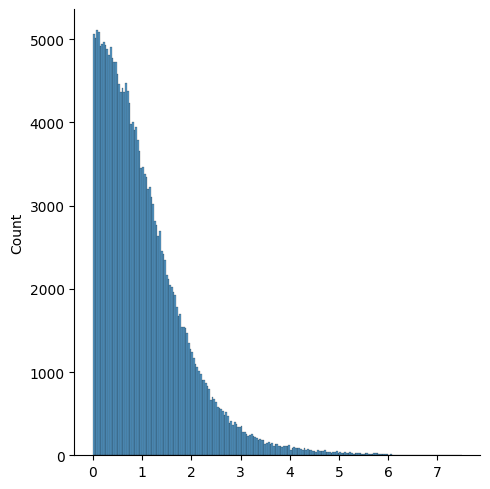
\includegraphics[scale=0.45]{titles.hist.png}
	}
	\subfigure[Hisogram błędu wraz z liczbą głosów]{
		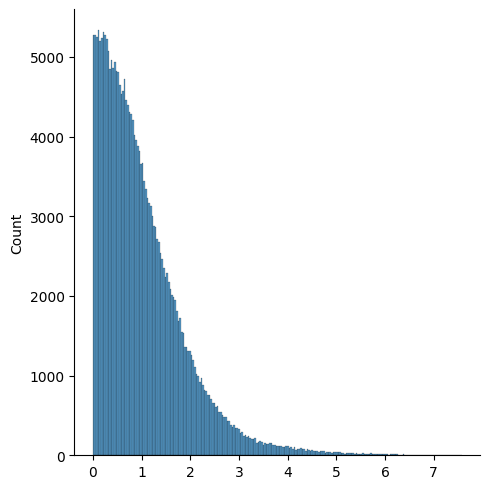
\includegraphics[scale=0.45]{titles-votes.hist.png}
	}
\end{figure*}

\begin{figure*}[htp]
\centering
	\subfigure[Porównanie bez liczby głosów]{
		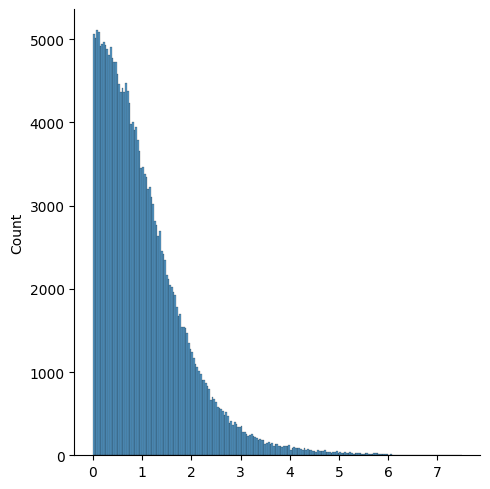
\includegraphics[scale=0.40]{titles.scatter.png}
	}
	\subfigure[Porównanie wraz z liczbą głosów]{
		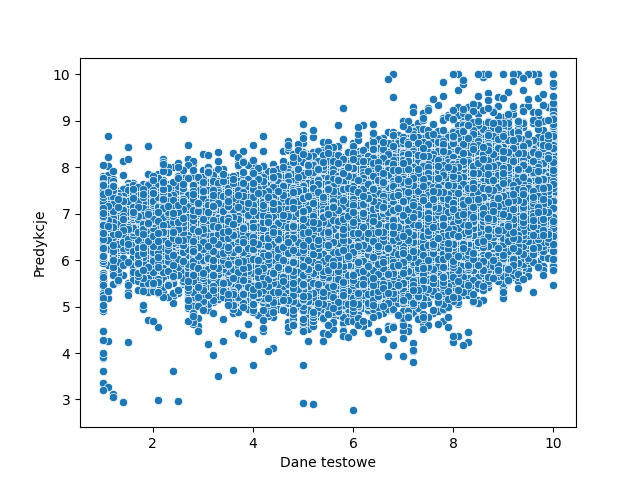
\includegraphics[scale=0.40]{titles-votes.scatter.png}
	}
\end{figure*}

\subsection{Gatunek oraz rok produkcji}

\sql{Łączenie oceny wraz z odpowiadającymi dziełu gatunkami oraz rokiem}{./queries/genres-year.sql}

\subsubsection{Rezultaty}

\begin{center}
\begin{tabular}{ |c|c| }
\hline	Średni błąd kwadratowy & \( 1.7144 \) \\
\hline	Najmniejszy błąd & \( 0.7 \times 10^{-5} \) \\
\hline	Największy błąd & \( 6.75 \) \\
\hline	Średni błąd & \( 0.994 \) \\
\hline
\end{tabular}
\end{center}

\includeplots{genres-year}

\section{Wnioski}

Głównym problemem niektórych z obranych metod może być dość niska zawartość informacji przenoszona przez wybrane dane do pradykcji (może tak być w przypadku np tytułu filmu). Koniecznym rozwinięciem projektu byłoby poszerzenie go o dalsze dane z serwisów jak TheMovieDB czy OMDB, które są kompatybilne z metodą indeksowania stosowaną w IMDB.

\subsection{Tabela zbiorcza rezultatów}

\begin{center}
	\begin{tabular}{ |p{0.15\linewidth}|p{0.15\linewidth}|p{0.15\linewidth}|p{0.15\linewidth}|p{0.15\linewidth}|  }
\hline Kwerenda & Średni błąd kwadratowy & Najmniejszy błąd & Największy błąd & Średni błąd \\
	\hline Tytuły filmów & \( 1.836 \) & \( 0 \) & \( 7.488 \) & \( 1.037 \) \\
	\hline Obsada & \( 1.272 \) & \( 0 \) & \( 7.310 \) & \( 0.82 \) \\
	\hline 3 głównych członków obsady & 1.375 & 0 & 6.882 & 0.8608 \\
	\hline 3 główni członkowie obsady i płeć & 1.353 & 0 & 7.788 & 0.853 \\
	\hline Tytuły i głosy & 1.803 & 0 & 7.573 & 1.024 \\
	\hline Gatunek oraz rok & 1.7144 & \( 0.7 \times 10^{-5} \) & 6.75 & 0.994 \\
	\hline
\end{tabular}
\end{center}

\end{document}
